%%
%% This is file `sample-manuscript.tex',
%% generated with the docstrip utility.
%%
%% The original source files were:
%%
%% samples.dtx  (with options: `manuscript')
%% 
%% IMPORTANT NOTICE:
%% 
%% For the copyright see the source file.
%% 
%% Any modified versions of this file must be renamed
%% with new filenames distinct from sample-manuscript.tex.
%% 
%% For distribution of the original source see the terms
%% for copying and modification in the file samples.dtx.
%% 
%% This generated file may be distributed as long as the
%% original source files, as listed above, are part of the
%% same distribution. (The sources need not necessarily be
%% in the same archive or directory.)
%%
%% The first command in your LaTeX source must be the \documentclass command.
%%%% Small single column format, used for CIE, CSUR, DTRAP, JACM, JDIQ, JEA, JERIC, JETC, PACMCGIT, TAAS, TACCESS, TACO, TALG, TALLIP (formerly TALIP), TCPS, TDSCI, TEAC, TECS, TELO, THRI, TIIS, TIOT, TISSEC, TIST, TKDD, TMIS, TOCE, TOCHI, TOCL, TOCS, TOCT, TODAES, TODS, TOIS, TOIT, TOMACS, TOMM (formerly TOMCCAP), TOMPECS, TOMS, TOPC, TOPLAS, TOPS, TOS, TOSEM, TOSN, TQC, TRETS, TSAS, TSC, TSLP, TWEB.
% \documentclass[acmsmall]{acmart}

%%%% Large single column format, used for IMWUT, JOCCH, PACMPL, POMACS, TAP, PACMHCI
% \documentclass[acmlarge,screen]{acmart}

%%%% Large double column format, used for TOG
% \documentclass[acmtog, authorversion]{acmart}

%%%% Generic manuscript mode, required for submission
%%%% and peer review
\documentclass[manuscript,screen,review,nonacm]{acmart}

\settopmatter{printacmref=false} % Removes citation information below abstract
\renewcommand\footnotetextcopyrightpermission[1]{} % removes footnote with conference information in first column
\pagestyle{plain} % removes running headers


%% Fonts used in the template cannot be substituted; margin 
%% adjustments are not allowed.
%%
%% \BibTeX command to typeset BibTeX logo in the docs
\AtBeginDocument{%
  \providecommand\BibTeX{{%
    \normalfont B\kern-0.5em{\scshape i\kern-0.25em b}\kern-0.8em\TeX}}}

%% Rights management information.  This information is sent to you
%% when you complete the rights form.  These commands have SAMPLE
%% values in them; it is your responsibility as an author to replace
%% the commands and values with those provided to you when you
%% complete the rights form.


%%
%% Submission ID.
%% Use this when submitting an article to a sponsored event. You'll
%% receive a unique submission ID from the organizers
%% of the event, and this ID should be used as the parameter to this command.
%%\acmSubmissionID{123-A56-BU3}

%%
%% The majority of ACM publications use numbered citations and
%% references.  The command \citestyle{authoryear} switches to the
%% "author year" style.
%%
%% If you are preparing content for an event
%% sponsored by ACM SIGGRAPH, you must use the "author year" style of
%% citations and references.
%% Uncommenting
%% the next command will enable that style.
%%\citestyle{acmauthoryear}

% Additional packages and commands used by this submission.

\usepackage{booktabs}
\usepackage{tabularx}
\usepackage{pdfpages}
\usepackage{ragged2e}
\usepackage{xcolor}

\graphicspath{{img/}}

\definecolor{blackwoodsblue}{HTML}{003B5C}
\definecolor{insightteal}{HTML}{008C95}
\definecolor{softgray}{HTML}{F2F5F7}

% Replace these two placeholders after importing the project into Overleaf and
% publishing the reproducibility repository.
\newcommand{\overleafprojecturl}{https://www.overleaf.com/read/tmpczntkxytf#f0247f}
\newcommand{\githubprojecturl}{https://github.com/Yaswanthgunti/blackwoods-customers-insights}

\newcommand{\wordcount}[1]{\noindent\textbf{[Word count: #1]}} %macro for word count

\newcommand{\todo}[1]{\textcolor{red}{\bf [[TODO: #1]]}} 

%extra packages for the tables in the appendix
\usepackage{longtable}
\usepackage{array}
\renewcommand{\arraystretch}{1.25}

\newcolumntype{Y}{>{\RaggedRight\arraybackslash}X}
\newcommand{\result}[1]{\textbf{#1}}

%%
%% end of the preamble, start of the body of the document source.
\begin{document}

%%
%% The "title" command has an optional parameter,
%% allowing the author to define a "short title" to be used in page headers.
\title{Customer Decision Intelligence for Blackwoods: Predicting Repeat Purchase and Session Conversion}

%%
%% The "author" command and its associated commands are used to define
%% the authors and their affiliations.
%% Of note is the shared affiliation of the first two authors, and the
%% "authornote" and "authornotemark" commands
%% used to denote shared contribution to the research.

\author{Yaswanth Gunti (s4188617)}
\affiliation{%
  \institution{RMIT University}
  \city{Melbourne}
  \country{Australia}}
\email{s4188617@student.rmit.edu.au}

%%
%% By default, the full list of authors will be used in the page
%% headers. Often, this list is too long, and will overlap
%% other information printed in the page headers. This command allows
%% the author to define a more concise list
%% of authors' names for this purpose.
\renewcommand{\shortauthors}{Gunti}

%%
%% The abstract is a short summary of the work to be presented in the
%% article.
\begin{abstract}
The current case study is designed for the Junior Data Scientist role in Blackwoods and is focused on assessing how the customer data impacts the decision-making process. Specifically, two freely available datasets were assessed independently but using the same timeframe for decision making, where previous purchases were used to predict further purchases, and the online session data was used to predict conversions. The regularized logistic regression was compared with the radial basis function kernel support vector machine.

\medskip
\noindent\textbf{Clickable Overleaf project URL:} \url{\overleafprojecturl}
\end{abstract}



%%
%% This command processes the author and affiliation and title
%% information and builds the first part of the formatted document.
\maketitle


%----------------------------------
\section{Data Science Role}
\label{sec:Data Science Role}
%----------------------------------

\subsection{Job Description and Role Identification}
\label{subsec:Job Description and Role Identification}

My choice for the \emph{Junior Data Scientist} position (job ref. 6721) from Blackwoods is a full-time entry level position within the Customer Experience Team’s Analytics Centre of Excellence. The advertisement has appeared on 6~August~2026 and will close on 5~September~2026. The position is advertised as located in Macquarie Park, NSW, but the job description says the work will be done from Blackwoods’ Sydney or Brisbane office~\cite{blackwoods2026job}.

This position requires working with business leaders to analyse complex datasets, find trends and causes, provide insight, use statistics and machine learning techniques in forecasting and resource management, and construct dashboards and visualizations. Programming languages such as Python or R, SQL and communication skills are needed; experience in Power BI and stakeholder interaction is preferred. These qualifications match very closely with my aspiration of providing insight that makes a difference in stakeholders' decisions. The full job listing is saved in the Appendix~\ref{sec:Job Listing}.

\noindent\textbf{Clickable job listing URL:}
\href{https://www.livehire.com/careers/blackwoods/job/DB9HM/1W7S2DP3U/junior-data-scientist}{Blackwoods --- Junior Data Scientist}


\subsection{Industry Context}
\label{subsec:Industry Context}

Blackwoods provides solutions within industrial and safety supplies. Data science contributes to both customer experience and commercial decisions through understanding purchase behavior, predicting demand and resource requirements, optimizing digital experiences, and interpreting operational data in ways that assist businesses with acquiring the appropriate products~\cite{blackwoods2026job}.

\wordcount{46}


\subsection{Role Focus}
\label{subsec:Role Focus}

The emphasis is on decision-oriented business insight backed up by prediction. In the ad, the focus is on trends, causes, insights, visualization tools for management; forecasting and machine learning are methods for resource allocation and prediction, not an end in itself~\cite{blackwoods2026job}.

\wordcount{44}


\subsection{Value Creation}
\label{subsec:Value Creation}

By understanding customer and operations trends, predicting demand, and offering decision-focused dashboards, the position can channel sales resources, optimize inventories and resource deployment, and eliminate friction in the customer journey. In turn, this will add value through improved decision-making, increased availability of products, more appropriate services, and reduced avoidable costs.

\wordcount{52}


\subsection{Values and Culture Alignment}
\label{subsec:Values and Culture Alignment}

I place great importance on clear explanations and constant learning, which coincide with Blackwoods’ claimed “Analytics Centre of Excellence” where information sharing is encouraged and a commitment to integrity, respect, and inclusiveness in the workplace exists. I would be able to provide clear analysis and welcome challenges from stakeholders~\cite{blackwoods2024sustainability}.

\wordcount{52}


\subsection{Diversity and Inclusion}
\label{subsec:Diversity and Inclusion}

The range of customers and communities served by Blackwoods calls for a wide range of analytics team members; this is because an inclusive team is more likely to challenge the limited nature of any assumption and identify overlooked demographics and behavior interpretation in the right context~\cite{wesfarmers2022diversity}.

\wordcount{49}


\subsection{Cover Letter}
\label{subsec:Cover Letter}

The customized cover letter appears in the final appendix section, which can be found on page \pageref{sec:Cover Letter}. It uses exclusively examples from my RMIT University data science courses and assignments, and not other part-time work experiences.

\wordcount{302}

%----------------------------------
\section{Data Set}
\label{sec:Data Set}
%----------------------------------

\subsection{Public Data Sets and Attributes}

\textbf{Dataset 1 --- UCI Online Retail:} 541,909 invoice lines from a UK non-store retailer (1~December~2010--9~December~2011), with eight recorded columns: invoice, product, description, quantity, date, unit price, customer ID and country. \textbf{Dataset 2 --- UCI Online Shoppers Purchasing Intention:} 12,330 web sessions with 17 predictors plus the Revenue target. Predictors capture page counts and durations, bounce and exit rates, page value, special-day proximity, month, operating system, browser, region, traffic source, visitor type and weekend. Both are publicly accessible and licensed CC BY~4.0~\cite{chen2015onlineretail,sakar2018onlineshoppers}.

\begin{itemize}
    \item \href{https://archive.ics.uci.edu/dataset/352/online+retail}{UCI Online Retail --- accessible dataset page}
    \item \href{https://archive.ics.uci.edu/dataset/468/online+shoppers+purchasing+intention+dataset}{UCI Online Shoppers Purchasing Intention --- accessible dataset page}
\end{itemize}

\wordcount{88}

\subsection{Selection Rationale}

They collectively complement the insight into customers, forecasting, and dashboarding aspects of the role across two time horizons. Retail transactions provide insights into future customers by predicting who will buy again, which helps in planning resource allocation. Session data provides insights into the conversion of visitors into buyers, highlighting any friction in the digital journey and visits with higher intent to buy. They are not combined as they pertain to different firms and departments.

\wordcount{74}

%----------------------------------
\section{Data Analysis}
\label{sec:Data Analysis}
%----------------------------------

\subsection{Decision Questions and Analytical Design}

This advertisement requires an analysis process that involves the conversion of complicated information into insights, forecasting, decision-making, and visualization~\cite{blackwoods2026job}. I have, therefore, formulated two questions for the stakeholders:

\begin{enumerate}
    \item Whom among existing clients must be prioritized by the account team since they have high potential for buying in the next 100 days?
    \item Which digital sessions indicate that there is purchase intent on the part of the client, hence their inclusion in journey monitoring or testing?
\end{enumerate}

These were modeled independently since they lack any common identifier and refer to distinct organizations. To merge them would create artificial relationships. However, these sources present two layers of customer decision support (Table~\ref{tab:design}) - medium-term planning of accounts and immediate prioritization of digital journeys.

\begin{table}[htbp]
\caption{Decision design after data-quality processing.}
\label{tab:design}
\small
\begin{tabularx}{\linewidth}{@{}Y Y r r@{}}
\toprule
\textbf{Source and unit} & \textbf{Binary outcome} & \textbf{Cases} & \textbf{Positive rate} \\
\midrule
Online Retail customer & Valid purchase, 1 Sep--9 Dec 2011 & 3,317 & 58.8\% \\
Online Shoppers session & Session generated revenue & 12,205 & 15.6\% \\
\bottomrule
\end{tabularx}
\end{table}

\subsection{Data Preparation and Leakage Controls}

\textbf{Customer repeat purchase.} The raw transactions data had 541,909 rows, including 5,268 exact duplicates and 135,080 rows without a customer ID. I discarded duplicates and transactions without a customer ID since repeating actions can't be linked to the customer. Invoices starting with ``C'' as well as non-positive quantities and prices were not considered as valid transactions. Cancellation-line rate was kept as a behavioural feature with history.

I applied 1~September~2011 as a temporal cut-off point. Valid transactions before the date led to the creation of 12 customer features: recency, the number and total price of orders, average price per order, quantity, average basket size, product diversity, active order days, observed tenure, average unit price, cancellation-line rate and UK flag. The target variable captures any valid transaction between 1~September~2011 and 9~December~2011. This design excludes future transactions from predictors and reflects the use of recency, frequency and monetary measures for customers~\cite{chen2012datamining}.

\textbf{Session conversion.} I removed 125 duplicate rows, resulting in 12,205 full sessions. The 17 provided predictors were kept, with \texttt{Revenue} being the target variable. The numeric variables were scaled, while the variables month, operating system, browser, region, traffic type, visitor type, and weekend were one-hot encoded. These predictors, according to the original study, are useful for predicting purchase intent in real time~\cite{sakar2019realtime}, but 
\texttt{PageValues} is proximate to the target, and thus its availability in real time needs to be confirmed first.

\subsection{Models and Validation}

Two classifiers were applied to each data source. Class-weighted, regularised \textbf{logistic regression} serves as a simple linear baseline. Class-weighted \textbf{radial-basis-function support vector machine (RBF SVM)} captures complex nonlinear relationships via a kernel function~\cite{cortes1995support}. RBF SVM is the classifier that is new for this assignment; it is not used in any of my previous machine learning assessments. The previous work involved decision trees, random forests, nearest neighbours, logistic regression, neural networks and XGBoost.

All the data processing took place within the pipeline of each model to avoid any data leakage from the hold-out test set into scaling and encoding procedures. A reproducible stratified 75:25 split with seed 42 left a separate test set untouched. Five-fold stratified cross-validation on the training set selected logistic-regression $C\in\{0.01,0.1,1,10\}$ and SVM $C\in\{0.5,1,5,10\}$ with $\gamma\in\{\text{scale},0.01,0.1\}$ according to the average precision score. The optimal classification threshold was chosen based on out-of-fold training scores. The test set was scored only once. The analysis is done using scikit-learn~\cite{pedregosa2011scikit}; the code and tables are provided in Appendix~\ref{sec:GitHub}.

To avoid mistaking a minor difference in number as an indication of significance, I performed 1,000 stratified bootstrap resamples for 95\% confidence intervals and a paired bootstrap interval to assess the difference in mean average precision between SVM and logistic regression. Permutation
importance calculated the drop in test average precision after 25 random permutations of each original feature.

\subsection{Evaluation Measures}

\textbf{Average precision (AP),} Summary of precision-recall curve, the key metric for model selection. It evaluates rankings regardless of thresholds and directly penalizes any dilution of true buyers among top ranks. This is particularly important for session conversion, which has only 15.6\% positive sessions; precision-recall performance is more meaningful than ROC on its own under class imbalance~\cite{saito2015precision}.

captures how many flagged cases end up buying, whereas \textbf{recall} captures how many buyers are flagged. The harmonic mean of these two values, \textbf{F1}, is an evaluation of the selected operating point by the training procedure, without letting the majority class accuracy have any upper hand. Accuracy and Balanced Accuracy were also verified but were not considered alone for model selection.

Lastly, \textbf{precision, lift and positive hits in the top 20\%} convert scoring into an implementation that is feasible for a capacity-limited stakeholder. Lift calculates the ratio of precision of the target group against the purchase rate of the entire population, while positive hits measure the proportion of all buyers in that particular target group.

\subsection{Model Effectiveness}

Table~\ref{tab:effectiveness} reports performance on held-out cases. Both algorithms discriminate future repeat purchasers moderately and session converters strongly. The session AP values are substantially above the 0.156 positive-rate baseline, and its ROC AUC is approximately 0.904. Figure~\ref{fig:performance} visualises the AP estimates and their bootstrap uncertainty.

\begin{table}[htbp]
\caption{Held-out performance. Brackets show 1,000-bootstrap 95\% intervals; threshold metrics use the F1-maximising threshold selected only from training data.}
\label{tab:effectiveness}
\scriptsize
\begin{tabularx}{\linewidth}{@{}Y l l r r r r@{}}
\toprule
\textbf{Outcome} & \textbf{Model} & \textbf{AP [95\% CI]} & \textbf{ROC} & \textbf{F1} & \textbf{Prec.} & \textbf{Recall} \\
\midrule
Repeat purchase & Logistic & .810 [.777, .844] & .736 & .748 & .631 & .920 \\
Repeat purchase & RBF SVM & .814 [.780, .846] & .736 & .748 & .606 & .977 \\
Session conversion & Logistic & .663 [.617, .710] & .904 & .647 & .594 & .711 \\
Session conversion & RBF SVM & .670 [.623, .718] & .904 & .649 & .604 & .700 \\
\bottomrule
\end{tabularx}
\end{table}

\begin{figure}[htbp]
    \centering
    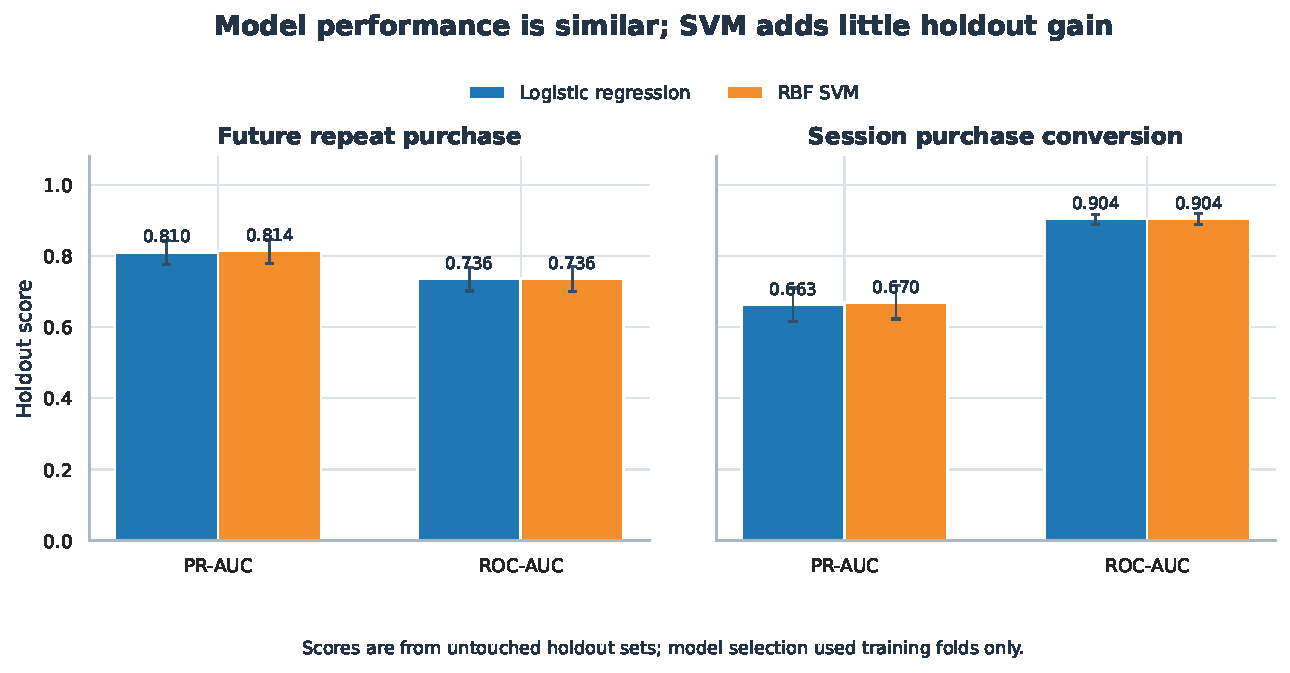
\includegraphics[width=\linewidth]{model_performance.pdf}
    \Description{Grouped bars compare average precision and ROC AUC for logistic regression and RBF SVM on repeat-purchase and session-conversion holdout sets. The bars and bootstrap intervals are nearly equal within each outcome.}
    \caption{Test-set model comparison. Error bars are 95\% bootstrap intervals.}
    \label{fig:performance}
\end{figure}

The advantage in terms of AP of the RBF kernel SVM for repeat purchases is just 0.0039 (95\% paired CI $[-0.0048,0.0125]$) and 0.0063 (95\% CI $[-0.0222,0.0361]$) for conversion. As these intervals contain 0, the analysis fails to confirm any reliable advantage of nonlinear models in this application setting. Repeat purchase F1 score is virtually equal. However, SVM discovers more repeat purchasers (97.7\% recall) at the expense of slightly lower precision (60.6\%) compared to logistic regression (92.0\% recall, 63.1\% precision). Thus, an optimal threshold will depend on the relative costs of false negatives and false positives rather than on classification accuracy.

The ranking results confirm this conclusion (Table~\ref{tab:lift}). In case of conversion, considering only the highest-scoring 20\% of sessions increases purchaser rate from 15.6\% to 56.8–57.6\%, identifying 73\% of purchasers, which is 3.6–3.7 times better than random targeting. Future repeat purchase has a higher base rate, so the lift is small but still valuable since the top quintile has a 90\% lift.

\begin{table}[htbp]
\caption{Decision value within the top-scored 20\% of held-out cases.}
\label{tab:lift}
\small
\begin{tabularx}{\linewidth}{@{}Y l r r r@{}}
\toprule
\textbf{Outcome} & \textbf{Model} & \textbf{Precision} & \textbf{Lift} & \textbf{Positives captured} \\
\midrule
Repeat purchase & Logistic & 89.2\% & 1.52$\times$ & 30.3\% \\
Repeat purchase & RBF SVM & 90.4\% & 1.54$\times$ & 30.7\% \\
Session conversion & Logistic & 56.8\% & 3.63$\times$ & 72.7\% \\
Session conversion & RBF SVM & 57.6\% & 3.69$\times$ & 73.8\% \\
\bottomrule
\end{tabularx}
\end{table}

\begin{figure}[htbp]
    \centering
    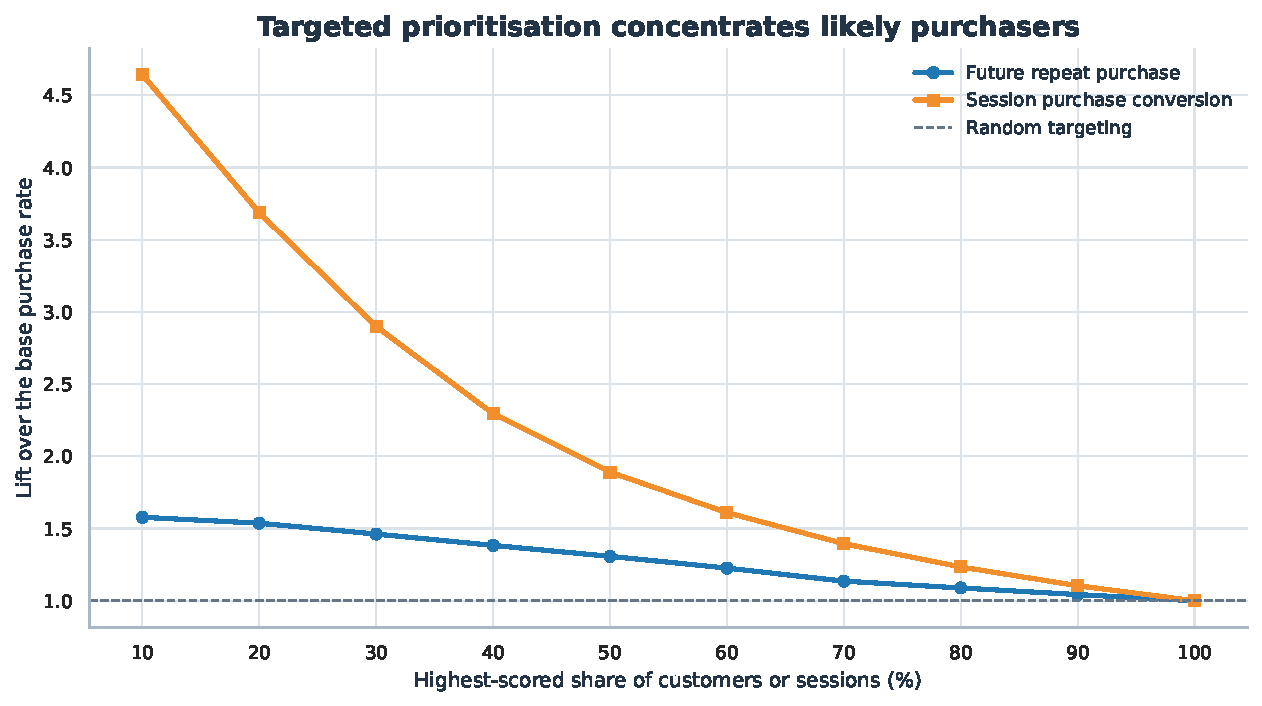
\includegraphics[width=\linewidth]{decision_lift.pdf}
    \Description{Two cumulative lift curves decline as the targeted share grows. Session conversion begins near 4.7 times the base rate at ten percent; repeat purchase begins near 1.6 times. Both reach one at the full population.}
    \caption{Cumulative targeting lift across progressively larger priority groups.}
    \label{fig:lift}
\end{figure}

\subsection{Insights from Both Sources}

\textbf{Longer-term customer signal.} The repeat purchase decreases monotonically with the quartile of recency: 77.8\% for the most recent quartile of customers (median of 13 days post-purchase), 66.7\% for the recent quartile of customers, 53.3\% for the lapsing quartile of customers, and 36.9\% for the least recent quartile of customers (median of 198 days). This makes intuitive sense to the stakeholders. Model importance is more detailed, as the RBF SVM considers the observed tenure of the customers as the most important (AP change of -0.057 upon shuffling), followed by active days (0.017). The logistic model is biased towards active days.

\textbf{Immediate session signal.} \texttt{PageValues} is the biggest in both models: its shuffle causes a reduction in AP of 0.430 for logistic regression and 0.457 for SVM. Purchase rate ranges from 3.9\% where page value is zero to 78.0\% at the top positive quartile. The next most important field is month, which has an approximate impact of 0.037 in AP for either model, while exit rate, bounce rate, admin pages and product page duration are less important.

\begin{figure}[htbp]
    \centering
    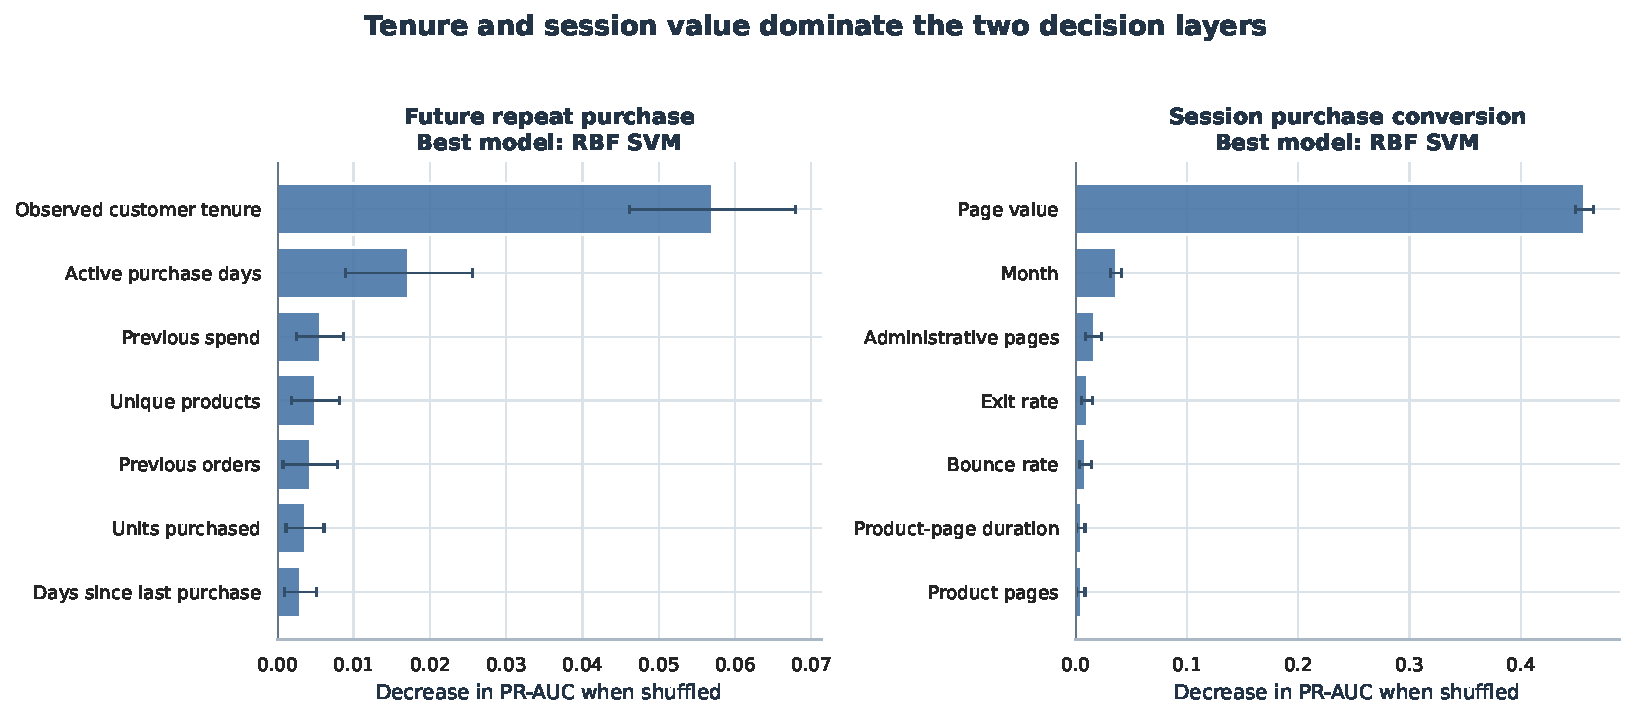
\includegraphics[width=\linewidth]{permutation_importance.pdf}
    \Description{Horizontal bars show that observed customer tenure and active purchase days lead repeat-purchase importance, while page value overwhelmingly leads session-conversion importance.}
    \caption{Permutation importance on held-out data, measured as decrease in AP.}
    \label{fig:importance}
\end{figure}

\begin{figure}[htbp]
    \centering
    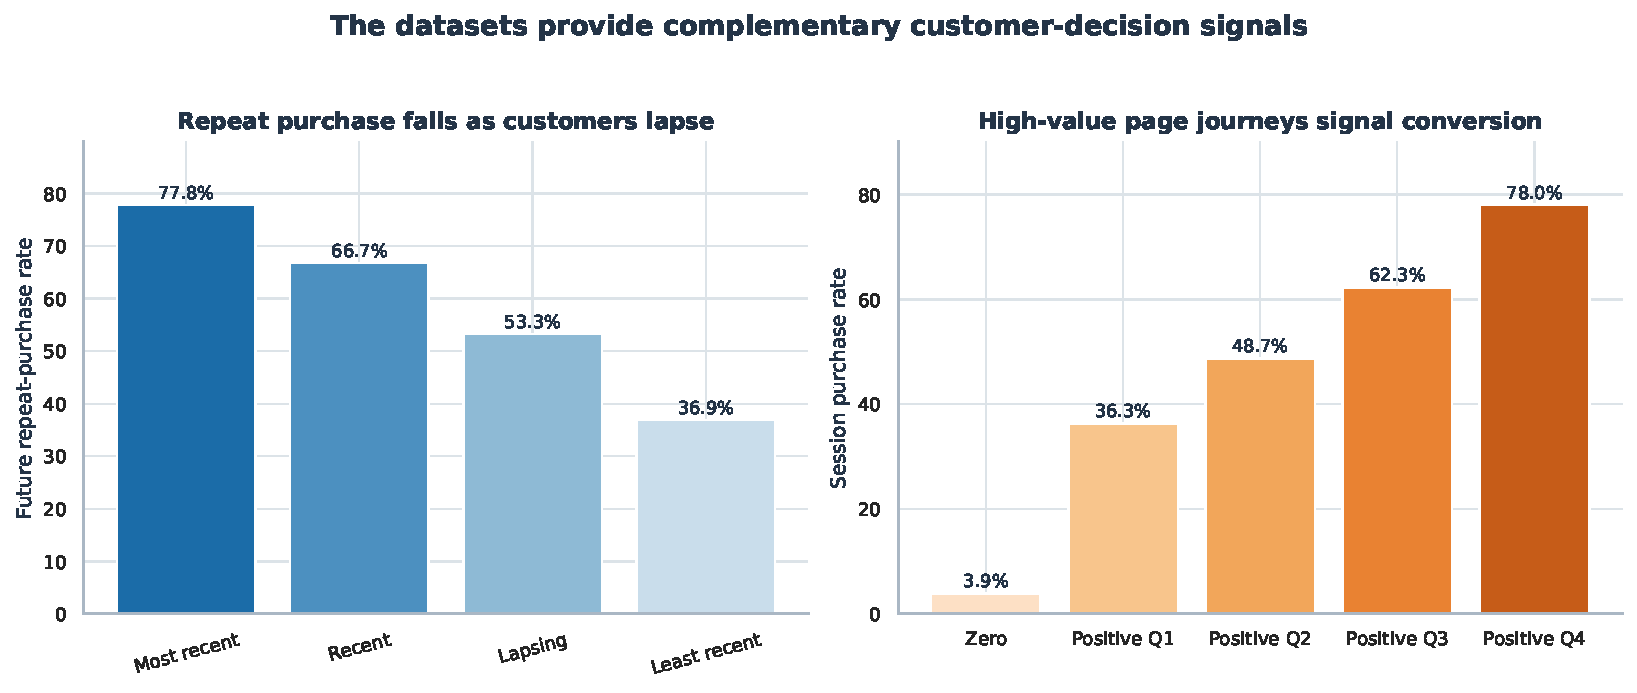
\includegraphics[width=\linewidth]{business_insights.pdf}
    \Description{Two bar charts show repeat purchase falling from 77.8 percent to 36.9 percent across recency groups, while session purchase rises from 3.9 percent at zero page value to 78.0 percent in the highest positive page-value quartile.}
    \caption{Descriptive patterns that make the two modelled decision layers interpretable.}
    \label{fig:insights}
\end{figure}

\textbf{Complementarity, not contradiction.} Insight is provided by both these sources. The transaction record gives information on durability of relationship and timing of re-engagement, while the session record gives information on intentions and conditions of the journey. The two records cannot confirm each other since they pertain to different organizations and organizational units, yet the messages they give are compatible – that engagement has been occurring recently and has high value, and so does the probability of a purchase.

\subsection{Recommendation, Governance and Limitations}

My recommendation is to use logistic regression as the production baseline model since there is no AP advantage demonstrated by SVM and the more complex model is harder to explain, monitor and challenge. The stakeholder dashboard would need to present score bands, base rate of the population, precision/lift of top-20\%, freshness of the data and the validation date of the model. The customer view can help with prioritization of accounts; the session view can help with aggregated journey monitoring.

In advance of its roll-out, the pipeline used by Blackwoods needs to be validated on data that is contemporary and particular to their organisation; all fields, in particular \texttt{PageValues}, need to be verified prior to the decision process. Calibration of the scores is required if there is a presentation of probabilities, while costs in terms of false positives and negatives have to be estimated. The trial has to take place as the predictive relationship does not prove the intervention effects.

The problem with external validity is another limitation. Online Retail has recorded UK gift sales during 2010 and 2011, not current Australian industrial supply sales, and anonymous customers are also ruled out. Online Shoppers includes anonymous customer log-ins without any time frame and demographic details. Therefore, representation and error differences between the different groups cannot be assessed. These data sets can be used only to illustrate how analysis can be performed and not for claims concerning Blackwoods customers.



\clearpage
%%
%% The acknowledgments section is defined using the "acks" environment
%% (and NOT an unnumbered section). This ensures the proper
%% identification of the section in the article metadata, and the
%% consistent spelling of the heading.
\begin{center}
    \noindent \textcolor{purple}{\emph{-- Content below this line does not count for the page/word limit. --}}
\end{center}

\section*{Generative AI Attribution and Declaration}
Condition~3 (Bounded Process) was used with OpenAI ChatGPT (Codex) in order to clarify task requirements, find public references, analyze Python and \LaTeX, debug code, and refine language and writing style. I have confirmed the references, performed the analysis, critically evaluated all recommendations, and am accountable for each claim and submission. The following is the Condition~3 declaration for this paper.

I certify that the submission of this assignment is incomplete without the submission of the completed \textbf{Condition 3 Bounded Process AI Declaration Form} (templates available in the specification of the assignment on Canvas).

\begin{acks}
I acknowledge the traditional custodians of this land, the Woi wurrung and Boon wurrung peoples of the eastern Kulin Nation, whose country RMIT University operates upon. I pay respect to their ancestors and elders, both past and present, and all those of their lands and waterways from which RMIT operates~\cite{rmit2026country}.
\end{acks}


%%
%% The next two lines define the bibliography style to be used, and
%% the bibliography file.
\bibliographystyle{ACM-Reference-Format}
\bibliography{99-references}

%%
%% If your work has an appendix, this is the place to put it.
\appendix
% Register Appendix A without creating a mostly empty title page. The embedded
% PDF itself names the role, carries the capture date and contains a clickable
% original-listing link in its footer.
\refstepcounter{section}
\phantomsection
\addcontentsline{toc}{section}{\protect\numberline{\thesection}Job Listing}
\label{sec:Job Listing}
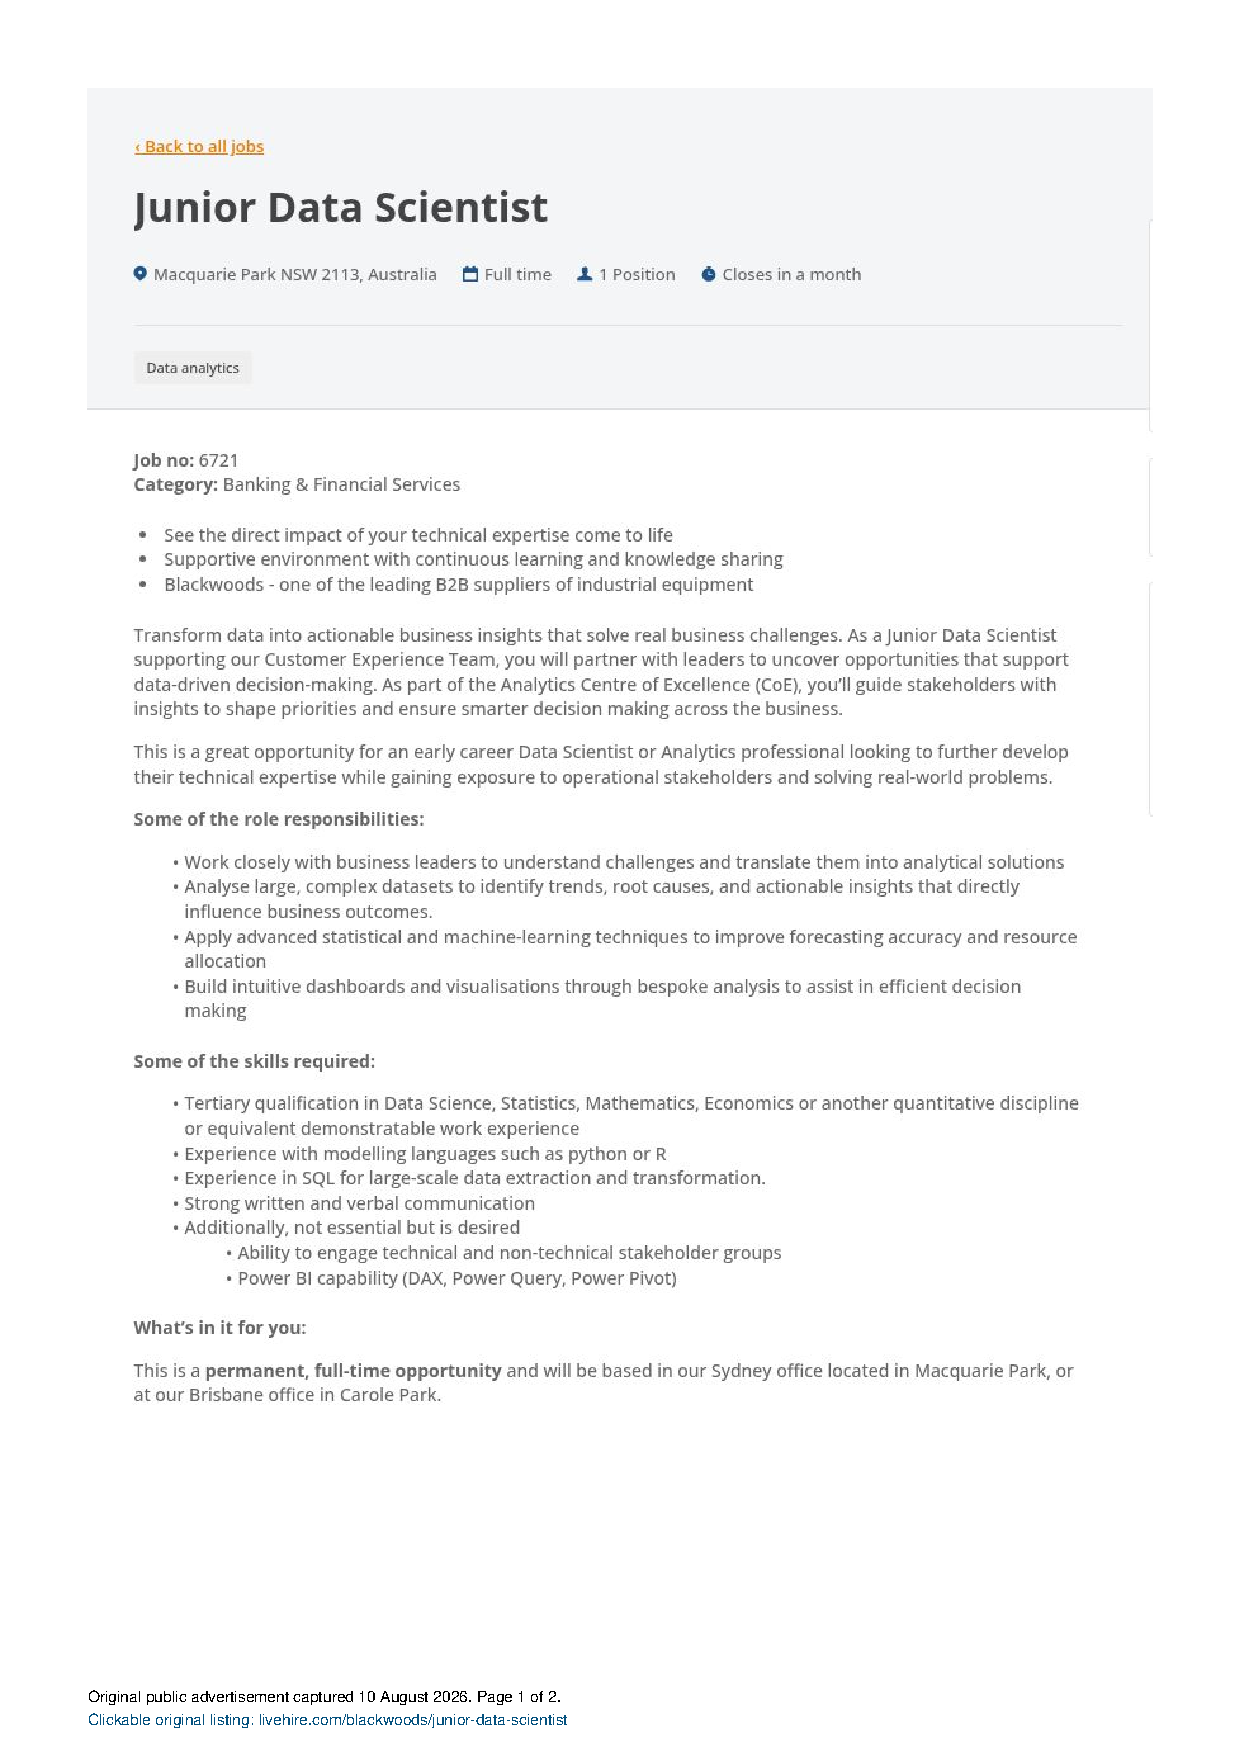
\includepdf[
  pages=-,
  fitpaper=false,
  pagecommand={\thispagestyle{plain}}
]{job_ad_blackwoods.pdf}


%----------------------------------
\section{Link to GitHub Repository}
\label{sec:GitHub}
%----------------------------------

\noindent\textbf{Clickable reproducibility repository:}
\url{\githubprojecturl}

Repository includes the full Python code, dependencies, data source information, processed data, output of models, and all figures used in this report. Raw public data is downloadable from UCI automatically; there is no private or Blackwoods customer data used.


% The cover letter is deliberately the final, unnumbered-looking page so it can
% be extracted and sent as a professional stand-alone letter while retaining an
% appendix label for cross-referencing from the report.
\clearpage
\refstepcounter{section}
\phantomsection
\addcontentsline{toc}{section}{\protect\numberline{\thesection}Cover Letter}
\label{sec:Cover Letter}
\thispagestyle{empty}

\begin{flushright}
\textbf{Yaswanth Gunti}\\
Melbourne, Victoria\\
\href{mailto:s4188617@student.rmit.edu.au}{s4188617@student.rmit.edu.au}\\[0.8em]
10 August 2026
\end{flushright}

\noindent Hiring Manager\\
Blackwoods\\
Macquarie Park, NSW

\medskip
\noindent Dear Hiring Manager,

\medskip
\noindent I am interested in the role of Junior Data Scientist (Vacancy No.~6721), which is available in the Customer Experience Team of Blackwoods. At present, I am enrolled in a Master of Data Science at RMIT University, which makes this role interesting for me.

\medskip
\noindent The RMIT projects illustrate the whole range of competencies that come with the job. The course on Practical Data Science includes preparing a dataset of 4,424 student outcomes, performing the analysis of classification models via cross validation and class sensitive measures and finally formulating actionable conclusions. The course of Advanced Programming saw me developing a reproducible Python process for extracting and integrating XML reviews data with handling of missing, inconsistent and duplicates. My Data Visualisation project using ABS General Social Survey data improved my R and Plotly skills and developed my storytelling capability.

\medskip
\noindent In this particular case study, I expanded upon this experience by analyzing 541,909 retail transaction records and 12,330 Internet sessions. In addition to feature engineering for customers and journeys, I compared regularized logistic regression with a nonlinear support vector machine, quantified uncertainties, and mapped predictions to targeting lifts. This project helped me hone my Python programming skills and data analytics abilities. Most importantly, however, it re-emphasized a critical lesson - a more complicated model should only be considered when providing decision value reliably.

\medskip
\noindent The values of Blackwoods with regard to collaboration, learning, inclusion, and direct impact of business align well with my working style. The Data Science Professional project that involved responsible application of a language model for finance taught me the importance of limitations, evidence, and communication. I would apply this approach in working with business leaders, while developing my skills in SQL and Power BI in the Analytics Centre of Excellence.

\medskip
\noindent It is with great interest that I would like to discuss the contribution that my analysis base, curiosity, and stakeholder-based communication would make toward decision making at Blackwoods.

\medskip
\noindent Yours sincerely,

\medskip
\noindent Yaswanth Gunti



\end{document}
\endinput
%%
